\documentclass[a4paper, 12pt]{article}
\usepackage[english]{babel}
\usepackage[pdftex]{graphicx}
\usepackage[latin1]{inputenc}
\usepackage[T1]{fontenc}
\usepackage{hyperref}
\usepackage{listings}


\setlength{\parindent}{0.0in}
\setlength{\parskip}{0.1in}

\setcounter{secnumdepth}{5}
\setcounter{tocdepth}{5}


\makeatletter
\renewcommand{\paragraph}{\@startsection{paragraph}{4}{0ex}%
   {-3.25ex plus -1ex minus -0.2ex}%
   {1.5ex plus 0.2ex}%
   {\normalfont\normalsize\bfseries}}

\renewcommand{\subparagraph}{\@startsection{subparagraph}{5}{0ex}%
   {-3.25ex plus -1ex minus -0.2ex}%
   {1.5ex plus 0.2ex}%
   {\normalfont\normalsize\bfseries}}
      \def\clap#1{\hbox to 0pt{\hss #1\hss}}%


\def\ligne#1{%
  \hbox to \hsize{%
    \vbox{\centering #1}}}%

\def\bovenaan#1#2#3{%
  \hbox to \hsize{%
    \rlap{\vtop{\raggedright #1}}%
    \hss
    \clap{\vtop{\centering #2}}%
    \hss
    \llap{\vtop{\raggedleft #3}}}}%

\def\onderaan#1#2#3{%
  \hbox to \hsize{%
    \rlap{\vbox{\raggedright #1}}%
    \hss
    \clap{\vbox{\centering #2}}%
    \hss
    \llap{\vbox{\raggedleft #3}}}}%

\def\maakvoorblad{%
  \thispagestyle{empty}\vbox to \vsize{%
    
    \bovenaan{}{}{}
    
    \vfill
    
    \hrule height 2pt
    \par
	  \begin{center}
	     \Huge \strut \@titel \par
	  \end{center}
    \hrule height 2pt
		\par

    \vspace{13mm}
    
    \ligne{\Large \@auteur}
    \vspace{5mm}
    \ligne{\@opleiding}
    
    \vspace{1cm}
    \vfill
    \vfill
    
    \onderaan{\@promotor}{}{\@academiejaar}
    }%
  \cleardoublepage
  }

\def\titel#1{\def\@titel{#1}}	
\def\auteur#1{\def\@auteur{#1}}
\def\opleiding#1{\def\@opleiding{#1}}
\def\academiejaar#1{\def\@academiejaar{Academiejaar: #1}}
\def\promotor#1{\def\@promotor{#1}}

\makeatother

%Default waarden
\auteur{Auteur}
\opleiding{Opleiding}
\titel{Titel}
\academiejaar{Academiejaar}
\promotor{Promotor}


\begin{document}
\auteur{Kwinten Missiaen, Steven Thuriot, Koen Van den dries, Bart Vangeneugden}
\opleiding{Methodologie�n voor Ontwerp van Programmatuur}
\titel{Taskmanager: Iteration 2}
\academiejaar{2009 - 2010}
\promotor{Tom Holvoet\\Mario Cruz Torres}

\maakvoorblad

\newpage
\thispagestyle{empty}
\mbox{}

\newpage
\maakvoorblad

\newpage

\tableofcontents

\newpage
\section{Introduction}
		This document serves as a documentation instrument for the first Iteration of the MOP Team Assignment.\\
		In the following chapters, the reader will get a general overview of the outer- and inner workings of the application, accompanied by several diagrams. At first, we will discuss the view layer. The user will be explained how the user interacts with the system. Delving deeper, we lay out how packages were used to ensure safe, decoupled and thought-through class-to-class communication.
		Once this is covered, we explain in detail just which classes have which responsibility, and why. Also our testing approach is explained in short.\\
		We conclude with our team organization, planning and a short self-evaluation.
	\section{System Operations}
		\subsection{Task Management}
			The system revolves around Tasks. There are many different entities to keep in mind such as Users, Resources or Projects.
			But all of these things somehow have to do with Tasks itself.
			\subsubsection{Creation of tasks}
				When creating a Task, the User asked to give details about the task at hand. The user is expected to enter a short description, the start time of the task, the deadline and the average duration of the task.
				Also, the user is presented with a list of resources and other tasks already in the system. The user then selects a few dependencies for the task he's creating and resources he wishes to allocate.

				When creating a task, the user has to make sure he does not violate the business rule when creating this Task. This means the user enters a duration, start date and end date. The start date must come before the end date and the difference between end- and start date has to be larger or equal then the duration. Also the systems tests if the entered description is an empty string. If this happens, an error is shown.\\
				\begin{figure}[H]
					\begin{center}
						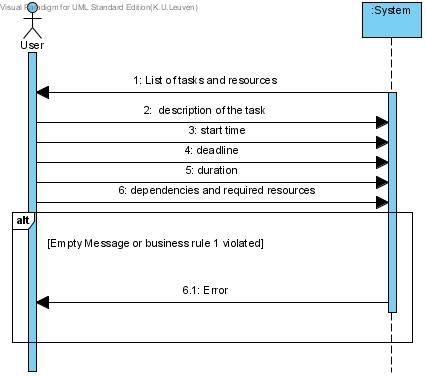
\includegraphics[scale=0.5]{images/ssd_create_task.jpg}
					\end{center}
					\caption{System Sequence Diagram describing the creation of a task}
				\end{figure}
			\subsubsection{Removing Tasks}
			When a task is to be removed. It first has to check how that will affect other entities in the system. Is a Task still required by other Tasks in a dependency?
			If this is the case. The user will receive an error message and is asked how he wants to proceed: Cancel the operation or delete all the dependent tasks.
			\begin{figure}[H]
				\begin{center}
					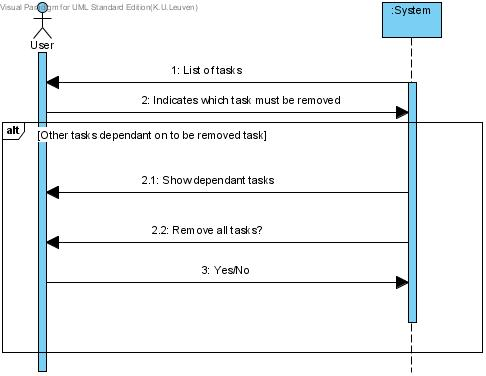
\includegraphics[scale=0.5]{images/ssd_remove_task.jpg}
				\end{center}
				\caption{System Sequence Diagram describing the removal of a task}
			\end{figure}
			\subsubsection{Modifying Tasks}
			When modifying tasks, the system has to make sure the user follows all the rules described above. This is because the user has the option to change all of the schedule variables, dependencies and required resources.

			This means that the Business Rule has to be tested, as well as the Empty Description rule. Checking is also done on the task dependencies. For instance, it should not be possible to create a task A, dependent on task B. And modify task B to be dependent on task A. This would create a dependency loop.\\
			\begin{figure}[H]
				\begin{center}
					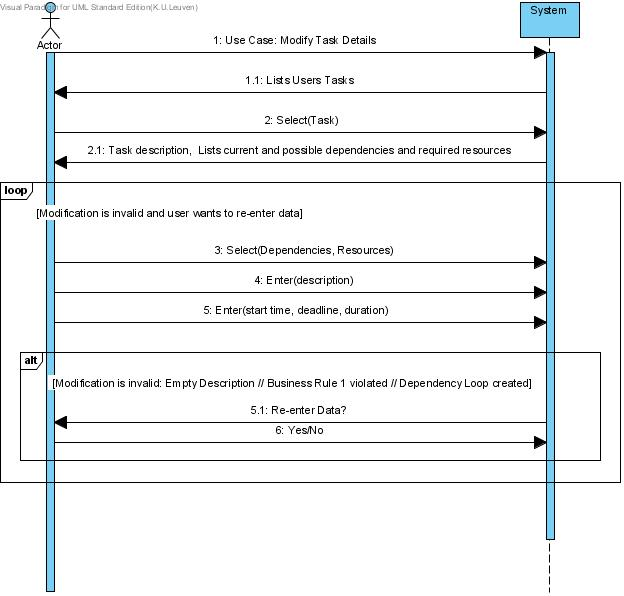
\includegraphics[scale=0.5]{images/ssd_modify_task.jpg}
				\end{center}
				\caption{System Sequence Diagram describing the editing of a task}
			\end{figure}
			 \subsubsection{Updating a Task status}
			Updating a status of a task is integrated in modifying a task, but requires special attention as many different rules apply when adjusting the status of a Task.

			Updating the status can directly reflect the status of dependent tasks. When a task was marked Successful, but is reverted to Failed or Unfinished the user will be asked to update the status of all dependent tasks or leave everything including this tasks status unchanged. This is because may have to revert back to Failed or Unfinished because they depended on the successful completion of this task.
			\subsection{Getting a task overview}		
			\emph{
			When asking for a overview of tasks, it is sometimes easy to sort and/or filter tasks in a different manner. That way you can get a better overview.\\
			We provided a handy interface for this in the way of a loop. The user can choose how he wants his tasks sorted: by deadline of by duration. In case the user selects to sort the tasks by deadline, he is asked how many tasks are to be shown. Is duration selected, a minimum and maximum duration is asked. It's made particulary easy to alter and/or add sorting and filtering methods.\\
			\begin{figure}[H]
				\begin{center}
					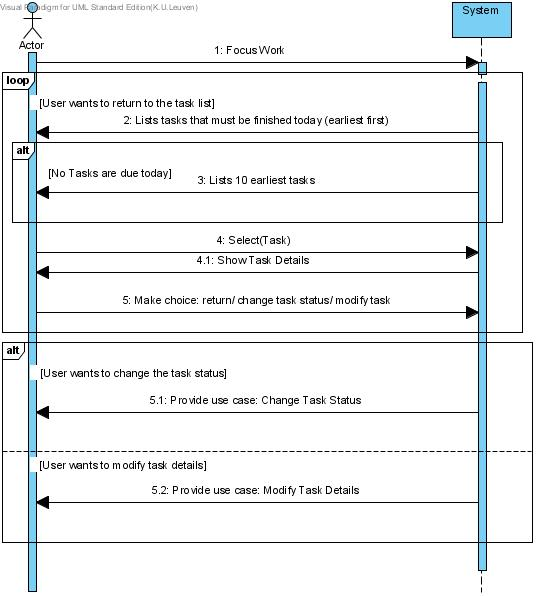
\includegraphics[scale=0.5]{images/ssd_focus_work.jpg}
				\end{center}
				\caption{System Sequence Diagram describing the overview of all tasks}
			\end{figure}
			}
			\begin{figure}[H]
				\begin{center}
					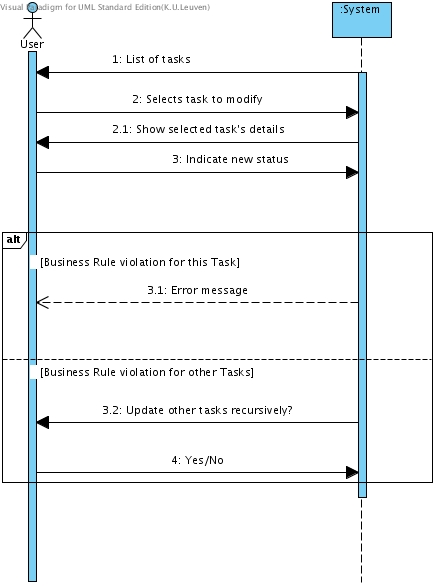
\includegraphics[scale=0.5]{images/ssd_update_task.jpg}
				\end{center}
				\caption{System Sequence Diagram describing the updating of the status of a Task}
			\end{figure}
		\subsection{Resource Management}
			\subsubsection{Creating Resources}
			A user can create a resource. When this resource is created, it is added to the system and stored there for later use.
			The system will only check for a valid description. This means the description can not be empty.

			Once created, the resource is available for binding to Tasks, or Reservations.
			\begin{figure}[H]
				\begin{center}
					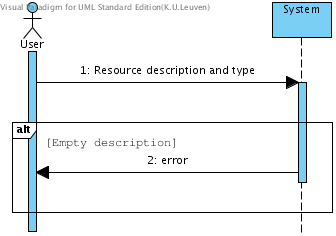
\includegraphics[scale=0.5]{images/SSD_Create_Resource.png}
				\end{center}
				\caption{System Sequence Diagram describing the creating of a new resource}
			\end{figure}
			\subsubsection{Remove Resource}
			A Resource can be removed. However, the system will first check it's dependency's with Task objects and/or Reservations.
			If the Resource is required by any of these, the system can not remove the Resource.
			\begin{figure}[H]
				\begin{center}
					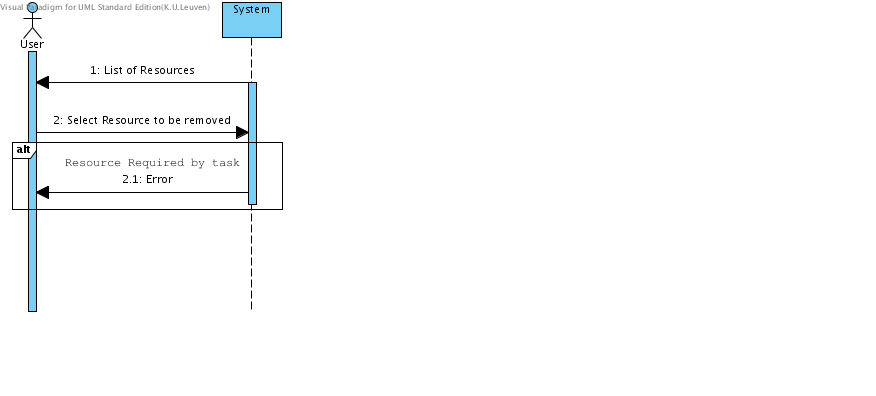
\includegraphics[scale=0.5]{images/SSD_Remove_Resource.png}
				\end{center}
				\caption{System Sequence Diagram describing the removing of a resource}
			\end{figure}
		\subsection{Reservations}
			\subsubsection{Create Reservations}
			Once a Resource is created, the User has the option to make a Reservation for that Resource.
			When creating a Reservation, the user is asked for the period of time he wants to make the Reservation after being shown a list of current Reservations for the Resource.

			After the user enters this data, the system controls the entered data to see if it does not conflict with previous Reservations.
			\begin{figure}[H]
				\begin{center}
					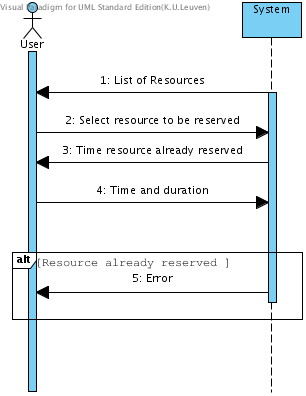
\includegraphics[scale=0.5]{images/SSD_Make_Resource_Reservation.png}
				\end{center}
				\caption{System Sequence Diagram describing the making of a reservation}
			\end{figure}
		\subsection{Project Management}
			\subsubsection{Create Project}
			A project can be created. A project can contain many Tasks, but does not have to. Our assumption is that at least one User is allocated to a Project, but several Users can subscribe.
			The system asks the user for a short description of that Project. If this description was not empty, the system creates the Project.
			\begin{figure}[H]
				\begin{center}
					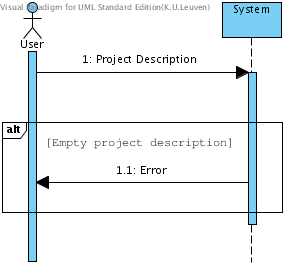
\includegraphics[scale=0.5]{images/SSD_Create_Project.png}
				\end{center}
				\caption{System Sequence Diagram describing the creating of a project}
			\end{figure}
			\subsubsection{Remove Project}
			A project can be removed without too many details. If the user wants to remove a project, all of the tasks connected to that project are removed. The user simply selects a Projects and all of the underlying tasks/dependent tasks are removed with it.
			\begin{figure}[H]
				\begin{center}
					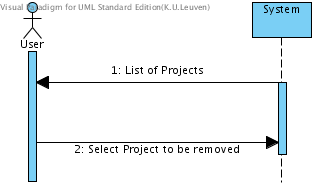
\includegraphics[scale=0.5]{images/SSD_Remove_Project.png}
				\end{center}
				\caption{System Sequence Diagram describing the removing of a project}
			\end{figure}
		\subsection{User Interface}
			\begin{figure}[H]
				\begin{center}
					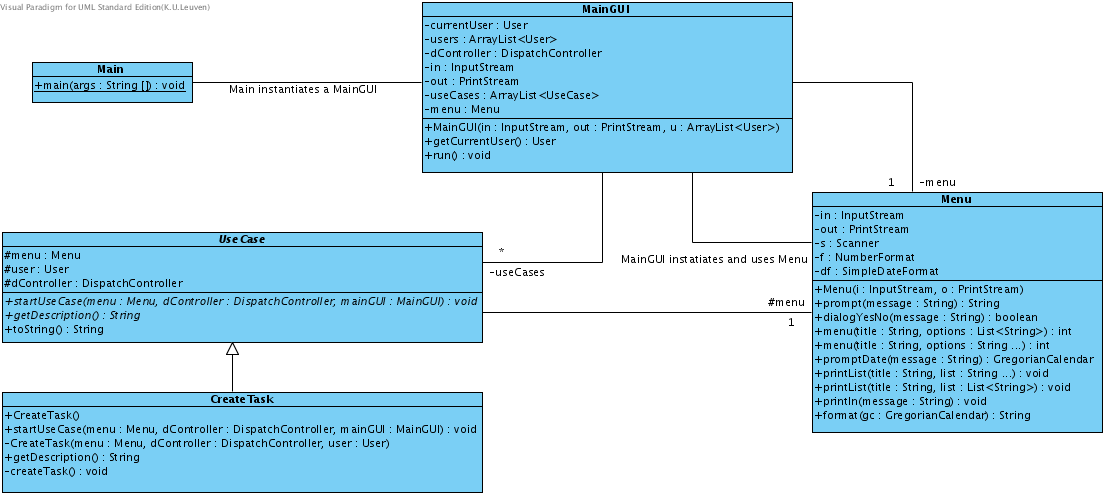
\includegraphics[width=1.0\textwidth]{images/gui.png}
				\end{center}
				\caption{Class diagram of the GUI}
			\end{figure}
			The project uses a text based UI. All use case are handled by a subclass of the abstract UseCase class, in the figure the use case for Create Task is given as example. MainGUI keeps a list of instance of these use cases. When the user initiates a use case MainGUI calls the corresponding use case, passing on the dispatch controller which will be discussed later, the use case then creates a new instance of itself with all field initialized to handle the rest of the use case. The class Menu handles the actual communication with the user through the console, formatting all the in and output.
			
	\section{Package Communication}
	       The whole project is divided in four big packages. These packages are 'model', 'controller' and 'gui'. The last package is 'test', which has been separated from the rest of the project for obvious reasons.
       
        We chose to create these packages so everything would be separated from each other. It would be bad practice to let the GUI access the model in a direct way, since this would mean even a small change could result in massive changes throughout the GUI. 
        
        This is where the controllers come in. They offer a way of communicating with the model. They basically contain a set of functionalities that are used throughout the program. These will then make the correct calls to the model. This way everything is handled without using direct calls, creating a more persistent system against changes throughout the model.
        
        All these controllers are finally instantiated inside one big container called the dispatch controller. This controller enables the GUI to just instantiate one controller. Its constructor will take care of the rest. The other controllers are stored inside it and can be accessed by calling the correct getters. All the controllers can then easily be passed along the different views using this one object.

	\section{Class Descriptions}
		
			\subsection{User}
			At first, we intended the User class to be responsible for the creation of Projects and Tasks, because a User object contains a list of Tasks and Projects that belong to that User. In the end, we chose not to do so. We felt that that the indirection was not necessary and that it might not benefit the cohesion of the User class.

			While not described in the project assignment, we assumed the system could become a multi-user system in the next iteration(s). We therefore based our design on this.

			Every User object is responsible for keeping track of the Tasks that belong to him. The system can ask the User object to return a list of these Tasks.

			\subsection{Task manipulation}
			%Design uitleggen. Ook de GRASP patterns erbij zetten
			Tasks are collected in the User. They contain a list of Resources the User might require to execute the Task.
			A Task has attributes which define it's own description, a Start and End time as well as a Duration.
			Also, a Task has a list of Tasks on which the Task may depend. This means the status of the Task at hand is dependent on the Status of it's dependent Tasks.\\
			Keeping Low Coupling and High Cohesion in mind, Task has the following responsibilities:
			\begin{itemize}
				\item{Keeping track of its name, start date, due date, duration and status}
				\item{Keeping track of the resources required to execute the task}
				\item{Keeping track of its dependencies. Dependencies are implemented as double bindings, so they should be kept consistent}
				\item{Checking for the business rule 1, 2 and 3 and preventing the construction of loops in the dependency scheme}
				\item{Updating the status of dependent tasks when necessary}
			\end{itemize}
			A Task is not an Information Expert or Creator of Resources. As described in the next chapter, a Resource has its own management.
			We do feel it is necessary for the Task to know about its Resources.\\
			However, a Task is Information Expert about Task itself. Therefore, we felt that the Task class should be responsible for enforcing the business rules, preventing the construction of dependency loops, and updating the status of dependent tasks when necessary (as described in the use case 'update task status').
			
			While designing, it was suggested that perhaps the Task class has two distinct responsibilities this way: one concerning its own details, and one concerning the way it interacts with other Tasks in the dependency graph. In the end, we chose to stick to one single Task class, as we felt that the cohesion of this class was sufficiently high.
			
			\subsubsection{Task dependency manager}
				\emph{
			In the second iteration, we chose to have a second object manage the dependencies of tasks. A new class TaskDependencyManager was created. A Task object aggregates an instance of TaskDependencyManager at all times. All operations that concern only dependencies are delegated to this object.}
			
			\emph{
			On one hand, this creates a strong coupling between the Task and the TaskDependencyManager classes. On the other hand, we felt that the Task class was getting too bloated, and that it was responsible for too many things. Delegating some operations to the TaskDependencyManager helps to improve the cohesion of the Task class.}
			
			\begin{figure}[h]
			\begin{center}
			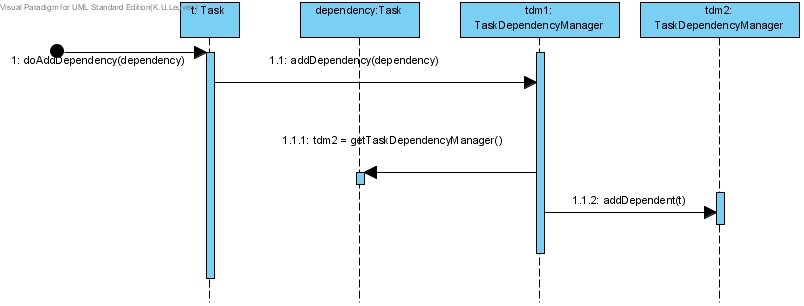
\includegraphics[scale=0.5]{images/doAddDependency}
			\end{center}
			\caption{\emph{Sequence diagram to add a dependency to a Task}}
			\end{figure}
			
			\emph{
			In the diagram is shown how adding a dependency to a Task works now. The Task object delegates this action
			to its TaskDependencyManager. The TaskDependencyManager then cooperates with the TaskDependencyManager of the second Task, to make sure the double binding is kept consistent.			
			Note: the diagram uses the operation 'doAddDependency()', not 'addDependency()'. This is because the operation 'addDependency()' is first delegated to the TaskState class. This is explained later in the report.}
			
			\subsection{Resource manipulation}
			%Design uitleggen. Ook de GRASP patterns erbij zetten
			Resources can be accessed via Tasks. This is because a Task can define which resources are required for that Task.
			However when a Resource is just created, or when a Task to which a Resource was allocated gets removed, the Resource will not be referenced to by any Task. The object would not exists.
			\emph{A resource is therefore stored in a RepositoryManager. This is explained in the section about 'Collecting Data'.}

			A Resource itself is an Information Expert as well as a Creator for Reservations. We decided to put the responsibility of creating and storing Reservations in Resource because a Resource needs this information to check it's own availability, as displayed in the diagram 'Create Reservation'.
			\begin{figure}[H]
				\begin{center}
					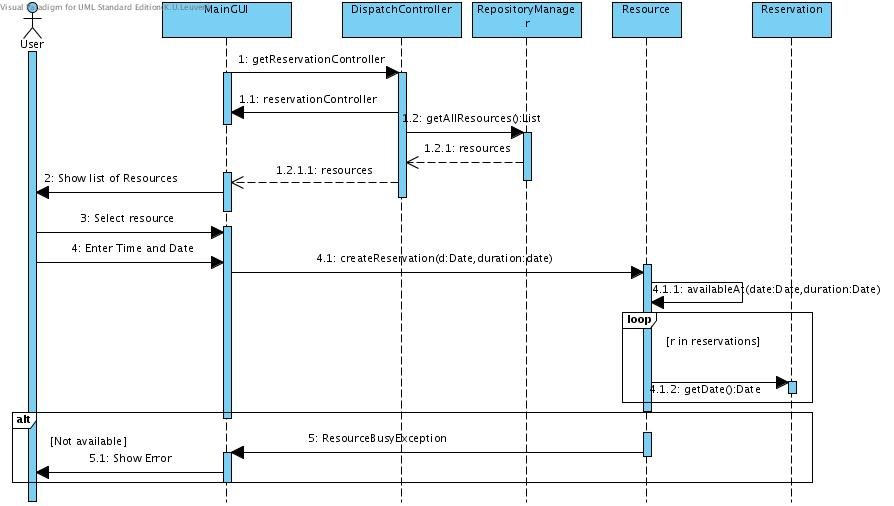
\includegraphics[scale=0.5]{images/create_reservation.jpg}
				\end{center}
				\caption{Create Reservation Sequence Diagram}
			\end{figure}
			
			
			\subsection{Project manipulation}
			\emph{A project is an instance that could contain Tasks. It does not have any binding to other objects and can not be stored in an object. Therefore, a Project is stored the same way a Resource is. By using repositories. See the subsection 'Collecting Data'.}
			\begin{figure}[H]
				\begin{center}
					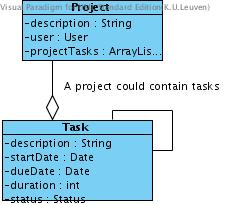
\includegraphics[scale=0.5]{images/project_class_diagram.jpg}
				\end{center}
				\caption{Project Class Diagram}
			\end{figure}
			
			The responsibilities of the Project class are as follows:
			\begin{itemize}
			\item Keeping track of its own details (description)
			\item Keeping track of the Tasks that are in the project
			\item Binding or removing Tasks from or to the project
			\end{itemize}

			\emph{Because an instance of type Project is not stored in any other domain class. We feel that none of these domain classes should therefore act as a Creator of the Project instances. We therefore opted to call the Project constructor in the controller, which then acts as a factory. This controller will also add the instance to the repositories.}
			
			\begin{figure}[H]
				\begin{center}
					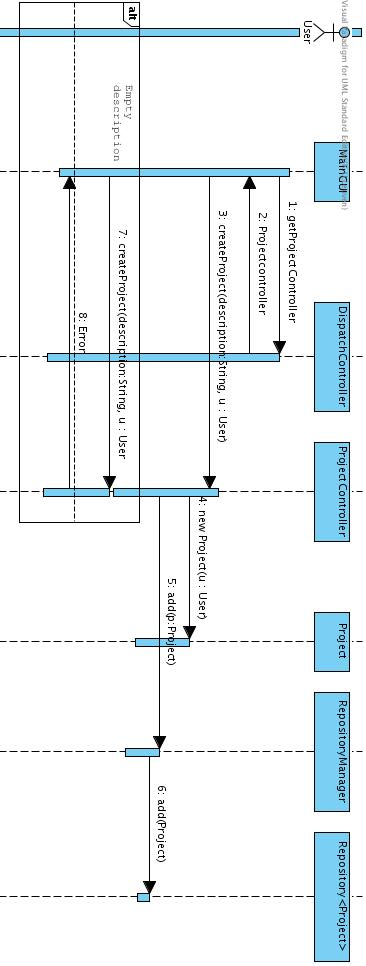
\includegraphics[scale=0.5]{images/create_project.jpg}
				\end{center}
				\caption{Create Project Sequence Diagram}
			\end{figure}
			\begin{figure}[H]
				\begin{center}
					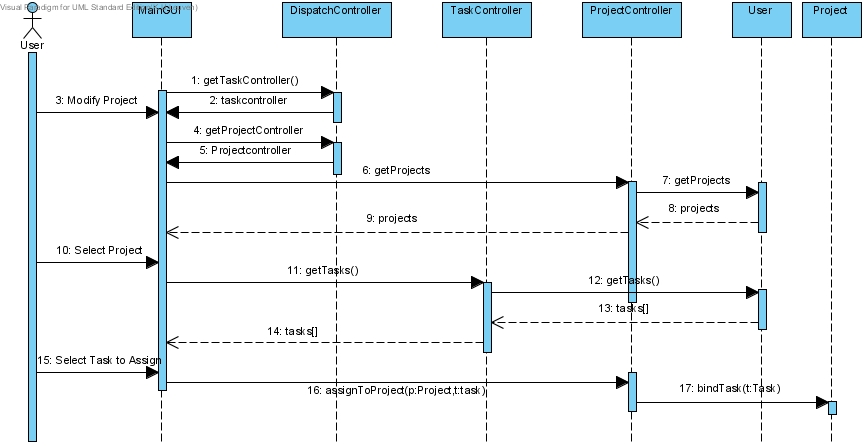
\includegraphics[scale=0.5]{images/assign_task_to_project.jpg}
				\end{center}
				\caption{Assign Task to Project Sequence Diagram}
			\end{figure}
			It is also the Project's responsibility to bind a Task to the Project. We feel that this direction should be maintained because a Project 'contains' or 'aggregates' a Task. This binding is done by calling a method in Project.
	
	\section{Software Structures}
		\subsection{Task states}
			\subsubsection{State Pattern}
				\emph{When receiving the new iteration, it instantly became clear that from now on states would play a big role in the design. Every state has its specific way of handling things. Without using a design pattern to solve this, the methods would become cluttered and unreadable really fast. They would also be very hard to maintain when states are removed or new states are created.}
			
				\emph{The perfect way to cope with all this is by using the state pattern. The state pattern offers all the functionality without having a lot of if structures inside the methods. This is done by creating an abstract class with all the methods from task that depend on the state of the task. By default, these methods get implemented in the abstract class so they throw an exception, saying the current call is not allowed in  the current state. This abstract class has one child for each possible state. The children will then overwrite the methods that they handle differently. As a result, the children will have a clear overview of all the methods that they allow, and have their own unique way to do so.}
			
				\emph{The task object has an instance of one of the children of the abstract state object. When one of these methods is called, the task object will simply redirect the call to the state object. Since the state object is a child, in other words a specific state, it will handle it in a correct manner for the current state.} 
			
				\emph{The state object also has a reference to the task object it belongs to. This is needed when the state needs to change. It is very important that the state pattern itself handles the state change. If this was not the case, separating all the states would become completely useless. This is because it is quite possible that a certain state would not allow to go to another state. In our case, for instance, it is not allowed to set a successful task back to unfinished.}
			
				\emph{We currently have four states, Available, Unavailable, Successful and Failed. Obviously, when a state is made, it will start out as either Available or Unavailable. Because the assignment was quite open about this, we had to think about what state changes we would allow throughout the system. We thought it would be best if Available and Unavailable were the only states that was allowed to change to another state. This would make it a lot easier for us to implement, because when a state would go from failed to available for instance, quite a lot of extra code is needed to figure out if the dependent tasks are failed because the the task you are changing was failed or for any other possible reason. In our current implementation, when, for instance, a task is failed and it needs to be changed, it is up to the user to create a brand new task. In the following diagram, you can see what state changes are allowed.}
				\begin{figure}[H]
					\begin{center}
						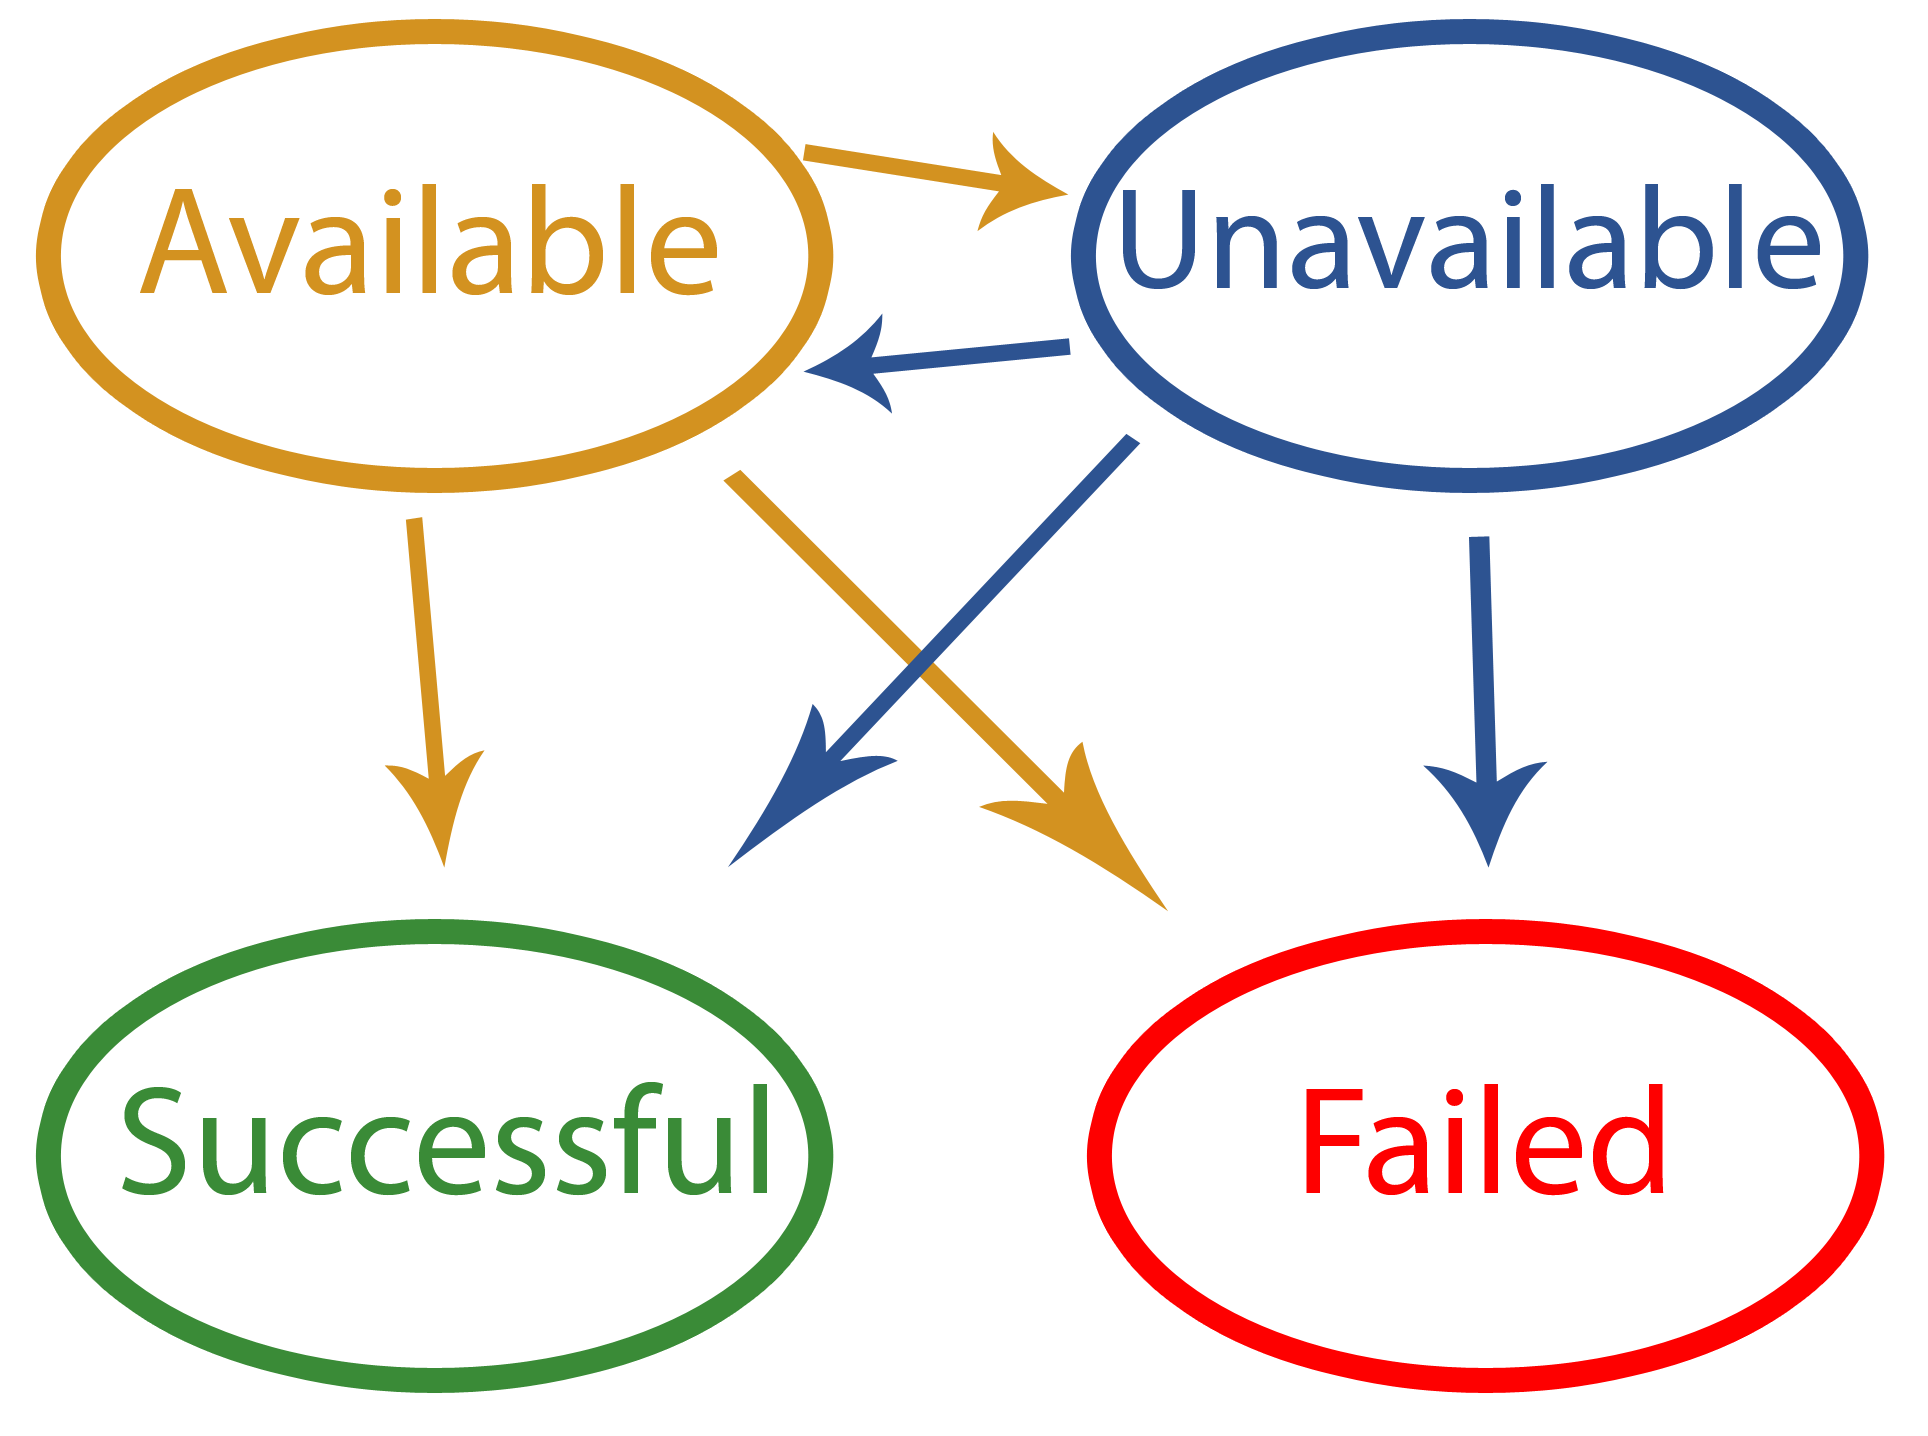
\includegraphics[scale=0.7]{images/StateChanges.png}
					\end{center}
					\caption{Assign Task to Project Sequence Diagram}
				\end{figure}
			
				\emph{As you can see are the state changes between Available and Unavailable the same. Because of this, we began to wonder what else was similar. After some thorough research, it became clear that the only difference between these two states was time related. Because of this, we decided to merge these two states into one big state, called "`Unfinished"'. This state would just calculate at runtime if it is available or not, and act accordingly. To eventually set the state, a method is added per state. There was also a parsing method created, to make it possible for the XML Parser to pass strings found in the XML file to the state. The state would then call one of the methods to change the state if it matches one of the existing states. If not, an exception is thrown. We decided to place this method into the state pattern itself, rather than the XML parser, because this way it is easier to maintain and harder to forget to adjust when a new state is made.}
			
				\emph{The original idea was to put Task, TaskState and all its children into a separate package inside the model package. Since all the methods used in TaskState are protected or private, rather than public, it would be impossible for any other class to call functions of the state. This however, was not possible. This is due to one of Java's limitations. Java has no "real" sub packages. They all count as different packages. Because of this, Java does not allow to call protected methods from a sub package. Sadly, this is exactly what some of Tasks methods needed to do. Because of this, we were forced to implement the state pattern inside the model package as well.}
						
			\subsubsection{Observer Pattern}
				\emph{In order to keep the states consistent across all tasks and dependencies we used the pull model observer pattern. At first, because one of the use-cases required to test which dependent task would change state as a result of the change of state of a task without actually changing the states, we considered using the push model. This would allow us to notify an observer of a state change, the new state where upon it would report back if and how it and it's dependent tasks would have changed state without changing state. This however would have limited the reusabilty of the observer pattern. But as the use-case requirement could be solved in the UI the observer pattern was reverted to the pull model. The two entities of the pattern are presented by the Subject and Observer<S extends Subject> interfaces using generics to improve reusabilty of the interfaces\footnote{Sadly, the type-erasure implementation of generics in Java only permits an interface to be implemented once by a class, even with different type arguments.}. As the Subject-Observer relationship is an implicit aspect of the task dependency relationship no subscribe(Observer) method is needed. While it is the TaskDependecyManager that maintains the dependency relationship we still chose to make Task both the Observer and Subject as it is Task that keeps the current state. When the state of a task is changed the publish() method is called to notify() all observing tasks, which will then decide whether they will update their own state. In order to comply with Business Rule 2 the observing task only needs to change status if the subject state is Failed. The update(Task subject) method of the observer is passed the subject which published the state change, but the observer still needs to verify if it is actually subscribed to the subject to ensure consistency.}
				
		\subsection{Task overview}
		\emph{
		As discussed, we want to show the list of tasks in different ways. We might want them sorted by deadline or by duration. However, there is no reason the functionality should be limited to just these two.\\
		Also, there is no reason to clutter the controller with these algorithms. We tried to find a way to split up the following functionalities:
		\begin{itemize}
			\item{Getting a list of tasks}
			\item{Sorting that list}
			\item{Filtering}
			\item{Returning the list}
		\end{itemize}
		We found our solution in the Strategy pattern: We start off by creating an instance of FocusWork. This instance is injected with an implementation of FocusStrategy and the current User.
		The instance of FocusWork will be responsible for getting the list of tasks. Since the sorting and filtering can differ from strategy to strategy, they are handled by the injected instance of FocusStrategy. That way, neither controller nor FocusWork (context) are responsible, or even aware, of how these algorithms work.\\
		There was however the issue of creating an instance of FocusWork. We found it bad design to let both GUI nor TaskController call the constructor of an implementation of FocusStrategy. This would mean higher coupling between those classes. It would also mean a larger footprint when adding new FocusStrategies, more classes had to be adjusted. We therefore opted for using the Factory Method pattern to create instances of FocusWork with an injected Strategy.\\
		The class FocusFactory takes care of Strategy constructors and injecting. The GUI now simply calls a method in this class, a pre-fabricated FocusWork is returned.\\
		All this combined makes sure that when we create a new implementation of FocusStrategy, the footprint is returned to a minimum: We have to adjust the GUI to make sure it asks the right questions, and the FocusFactory is adjusted so right constructor is called in the right way.\\
		\begin{figure}[H]
			\begin{center}
				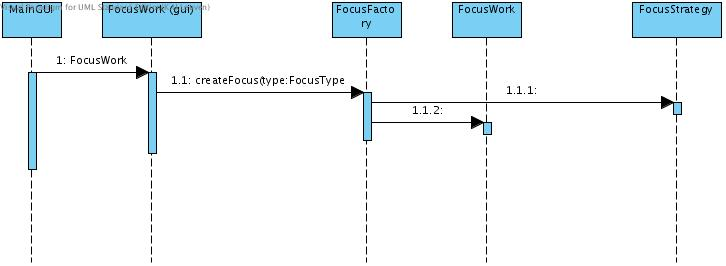
\includegraphics[scale=0.5]{images/FocusFactory.jpg}
			\end{center}
			\caption{Create a type of FocusWork with an injected Strategy according to a given Type}
		\end{figure}
		\begin{figure}[H]
			\begin{center}
				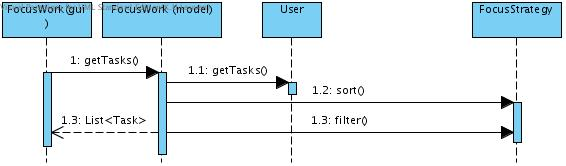
\includegraphics[scale=0.5]{images/FocusStrategy.jpg}
			\end{center}
			\caption{Get a list of tasks, manipulated by a certain Strategy. This strategy is interchangeable}
		\end{figure}
		\begin{figure}[H]
			\begin{center}
				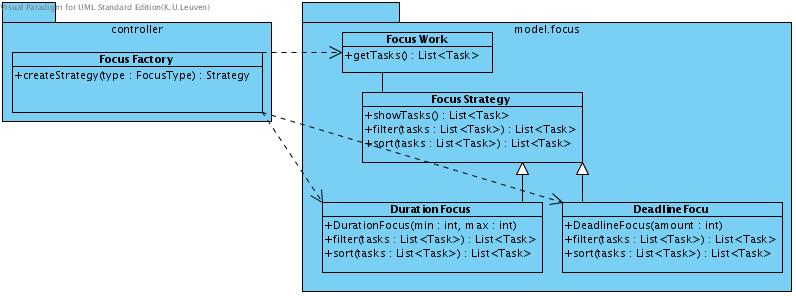
\includegraphics[scale=0.5]{images/focus_class_diagram.jpg}
			\end{center}
			\caption{Specialised class diagram explaining the Strategy Pattern}
		\end{figure}
		}
		\subsection{Linking Tasks by dependency}
		Uitleggen hoe tasks gelinked worden zonder te veel binding = taskdependencymanager
		
		\subsection{Time representation}
		\emph{
		Because Business Rule 3 relates so strongly to time, it seems natural to look for a way to represent time in our software system. As time progresses, the status of a Task may have to be changed to satisfy Business Rule 3. For example, if the deadline of a Task has passed and it wasn't finished yet, the Task was failed. This leaves us with two questions. How should we represent time in our system? How should we design the system so that Business Rule 3 can be uphold for all tasks at all time?}
		
		\emph{
		To represent time, we created a class 'Clock'. This class represents a certain moment in time, and supports a few very basic operations, such as setTime() en getTime(). If necessary, this class can easily be expanded later to allow for more complex behavior.
		An instance of Clock is created when the system is started. This object is stored in the RepositoryManager (see next section) and is passed on to every Task that is created. As such, the Tasks can use this object to get the current system time. This allows them to check for Business Rule 3.}
		
		\begin{figure}[h]
		\begin{center}
		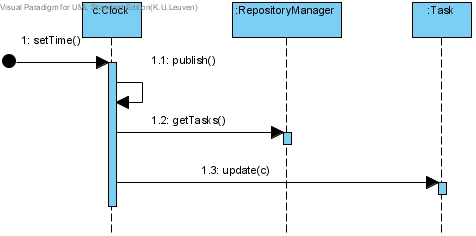
\includegraphics[scale=0.6]{images/setTime}
		\end{center}
		\caption{\emph{Set time sequence diagram}}
		\end{figure}
		
		\emph{
		Of course, checking for Business Rule 3 is not enough. The system must make sure that Business Rule 3 is satisfied at all times. This means that Tasks must check Business Rule 3 whenever the time changes, and if necessary, change their status accordingly.
		To accomplish this, we used the Observer pattern, as shown in diagram 'Set time sequence diagram'.
		Whenever the operation 'setTime()' is called, the Clock object calls another operation 'publish()'. Next, the Clock object asks the RepositoryManager for a list of all Tasks (see next section), and calls 'update(this)' on all of them. The Task is now notified that the current system time has changed. It is now the responsibility of a Task object to reach a consistent state.}
		
		\emph{
		We assumed that time can only go forward. Whenever 'setTime()' is called with a time before the current system time, an exception is thrown. This assumption seems very reasonable, and it greatly simplifies the behavior of the Clock and Task classes. A possible downside is that the system and its user interface may become less error friendly. If, by accident, the time is set in the distant future, it will be hard to revert this change.}
		
		\subsection{Collecting data}
		Certain types of objects (Resources, Projects) are not required to have a binding with other objects. They can be simply instantiated on their own.\\
		In a domain based model, this was a problem. Objects would be instantiated without a place to put them, they would not be contained. In the first iteration, we solved this by using a Singleton manager for Resource. Projects would be bound to a User.\\
		This seemed bad design, as Singleton was unreliable as an Information Expert. It was too general and would fail in most Unit tests. Storing the Project in the User also seemed bad design, as they originally had no connection to each other.\\
		A solution was found in using Repositories. We created Generic Repositories for Project, Resource and User that were contained in a RepositoryManager. The RepositoryManager would act as an independent Information Expert and would manage objects in adding and removing them from their respective repositories.\\
		By using overloaded add() and remove() operations, this RepositoryManager stayed easy to use and kept the underlying code abstract. We call this the Facade Pattern.\\
		We use a technique borrowed from the Spring Framework called Dependency Injection to inject a reference to this RepositoryManager in every Controller. This way, they can all access the same information in an Object-Oriented Way.
		
	\section{Software Initialization}
	\emph{When the program initializes, the first thing that gets created is the RepositoryManager. This makes sure repositories are created for Project, Resource and User. This also makes sure a Clock is created and contained.}
	
	After that, an XML parser object is created to retrieve all the supplied information. The dispatch controller, together with the location of the XML file, are passed to the constructor of the parser. After this it can finally start parsing.
	
	The first thing it will do is find all the resources in the file. It will then instantiate the ResourceManager singleton and start adding these resources. Once that has been completed, it will start looking for projects. It will create all the found instances. After this it looks for all the tasks and, once again, creates them all. Finally all the tasks, resources and projects are bound according to the specifications in the XML file. It will finally return the user object found in the file.
	
	After this the GUI is instantiated. The user object from before is passed along with its constructor and then starts listening for any input. 
	
	The system has now fully started and is ready for use.	
	
	
	\section{Testing}
		\subsection{Technology}
		We decided to use JUnit4 for testing.
		JUnit4 has a few advantages compared to JUnit3. It uses annotations to define a Test. This gives the developer an easy solution to testing for Exceptions.
		\subsection{Testing Approach}
		We decided to go for a defensive and multi-level testing approach.
		By multi-level we mean that we test both methods in Model classes (such as User, Task, Resource etc.) as well as testing the Controllers that call these methods (TaskController, ResourceController etc). 
		This way we get a good view on where errors are: model, controller or view.\\
		We also tested most methods for both cases. This means that we test both failure and succession of a method. Testing only for success does not guarantee a correct Exception is thrown, or success in all cases.
	\section{Project Management - Iteration 1}
		\subsection{Planning}
		Our Team Assignment had the following planning in iteration 1:\\
		\begin{tabular}{p{200 pt}|c|c}
		Activity & From & To\\
		\hline
		First meeting \& Discussion of our views on the project & 9/10/2009 & 9/10/2009\\ \hline
		Creation of a draft class diagram \& working out System Sequence Diagrams & 9/10/2009 & 12/10/2009\\ \hline
		First meeting with our advisor. & 12/10/2009 & 12/10/2009\\ \hline
		Individual rework of Class Diagram & 12/10/2009 & 14/10/2009\\ \hline
		Comparing results and creation of definitive Class Diagram & 14/10/2009 & 14/10/2009\\ \hline
		Creation of Sequence Diagrams & 14/10/2009 & 16/10/2009\\ \hline
		Development of Model classes and Controller classes. Building of GUI structure & 16/10/2009 & 19/10/2009\\ \hline
		Code review by team and rewriting certain functionality's & 19/10/2009 & 26/10/2009\\ \hline
		Start writing report \& finishing UML diagrams & 24/10/2009 & 27/10/2009\\ \hline
		\end{tabular}
		\emph{
			Our Team Assignment had the following planning in iteration 2:\\
			\begin{tabular}{p{200 pt}|c|c}
			Activity & From & To\\
			\hline
			TODO: planning
			\end{tabular}		
		}
		\subsection{Teamwork}
		We focused on a close teamwork. We started the project with a team discussion on how everyone saw the project and interpreted the assignment. This gave the team a general perspective and good grasp on how we wanted to implement it.\\
		We have 3 weekly physical meetings, where 1 would be with our team advisor. In these meetings, we discussed what everyone had done in the past days. Whenever somebody was unclear, or the group had doubts about which method or pattern would be the best to use, time was never an issue to come to a general solution that seemed best to everyone.\\
		We also used several team collaboration tools provided by Google such as Google Code and Google Groups. This gave advantages such as a mailing list, subversion with the option to review code at each revision, issue lists and hosted files.\\
		We tried to keep all the information as centralized as possible by using a separate Subversion repository for the Visual Paradigm file. This way every team member always had the most up to date diagrams available.\\
		Development of the project was divided in 4 groups of functionality: Controllers, Models, View and Testing. Each member of the team was assigned one of these tasks. Steven Thuriot took on Controllers and the parsing of XML, Kwinten Missiaen Models, Koen Van den dries the View and Bart Vangeneugden Testing. The report was structured and drafted by Bart Vangeneugden however every team member wrote about the part of development he was responsible for.\\
		\subsection{Timing}
		\textbf{Iteration 1:}
		We had a total of 18 hours meeting physically for the project. Besides that every group member worked at home. A short estimate follows:\\
		 \begin{tabular}{l|l}
		Member & Time(+/-)\\ \hline
		Kwinten Missiaen & 30\\
		Steven Thuriot & 25\\
		Koen Van den dries & 23\\
		Bart Vangeneugden & 25\\
		\end{tabular}
		\textbf{Iteration 2:}
		We had a total of XX hours meeting physically for the iteration. Besides that, every group member worked at home: A short estimate follows:
		\begin{tabular}{l|l}
		Member & Time(+/-)\\ \hline
		Kwinten Missiaen & 18\\
		Steven Thuriot & 25\\
		Koen Van den dries & 23\\
		Bart Vangeneugden & 14\\
		\end{tabular}
	\section{Self-Evaluation - Iteration 1}
	It is our opinion that we had a great team effort. However, we can improve. In this iteration we were too eager to get a first version of Class- and other diagrams ready. It would have been a better choice to make a good class-per-class analysis before drawing.\\
	To conclude we had no real problems regarding teamwork. Also we learned a lot about project organization.
	\section{Project Management - Iteration 2}
		\subsection{Planning}
		The planning of our Team Assignment had the following planning:\\
	
		\begin{tabular}{p{300 pt}|c}
		Activity & Date\\
		\hline
		First meeting to discuss the new iteration, discussion about the state pattern, observer pattern, the business rules and a new way to implement FocusWork. & 20/11/2009\\ \hline
		Adjusting parts of the class diagram \& System Sequence Diagrams to use the state pattern. & 25/11/2009\\ \hline
		Discussion about splitting task into two objects because it is currently bloated. Decided on using the strategy pattern for FocusWork. & 27/11/2009\\ \hline
		Discussed two options of splitting task. Decided on making a new class that is an attribute of task. & 30/11/2009\\ \hline
		Talked about the best way to implement some parts of the state pattern. Discussed making a generics wrapper so GUI has a describable but can't touch the actual objects. & 07/12/2009\\ \hline
		Discussed some code issues and set up some deadlines for the code and the report. & 11/12/2009\\ \hline
		Start writing report \& finish polishing up the UML diagrams & 16/12/2009\\ \hline
		Finish the report and go over it one more time as a team. & 18/12/2009\\ \hline
		\end{tabular}
		
		\subsection{Teamwork}
		
		
		We had a total of 16 hours meeting physically for the project. Besides that, every group member also worked at home. A short estimate follows:\\
		 \begin{tabular}{l|l}
		Member & Time(+/-)\\ \hline
		Kwinten Missiaen & 18\\
		Steven Thuriot & 18\\
		Koen Van den dries & --\\
		Bart Vangeneugden & --\\
		\end{tabular}
	\section{Self-Evaluation - Iteration 2}
	Just like last time, we had no real problems regarding teamwork. We also applied the same strategy. Meeting often and working hard.
	
	We divided the actual code among us, so it would be manageable to work on. Kwinten took care of making the time controller, the clock and the task dependency manager. Steven handled implementing the state pattern. Koen worked on the observer pattern, the describable wrapper and the GUI. Bart also worked on the GUI, but he also implemented the strategy pattern and the repositories. Finally, we all worked hard on writing tests and adjusting the UML diagrams.
	
	Everything was discussed thoroughly and everyone put in his best effort to try and make this iteration a success as well.
\end{document}
